\documentclass[10pt,twocolumn]{article}

\usepackage{verbatim}
\usepackage{listings}
\lstset{
    basicstyle=\footnotesize\ttfamily,
    columns=fullflexible,
    keepspaces=true,
    captionpos=b,
    aboveskip=6pt,
    belowskip=6pt,
    xleftmargin=1em,
    frame=single,
    framesep=4pt,
    numberstyle=\tiny,
}
\lstdefinestyle{numbered}{numbers=left, xleftmargin=2em}
\renewcommand{\lstlistingname}{Listing}
\usepackage{url}
\usepackage{graphicx}
\graphicspath{{imgs/}}

\usepackage{xspace}
\newcommand{\FC}       {Freechains\xspace}
\newcommand{\R}[1]     {rule~\code{#1}\xspace}
\newcommand{\reps}     {\emph{reps}\xspace}
\newcommand{\nreps}[1] {\emph{#1~reps\xspace}}
\newcommand{\code}[1]  {\texttt{\footnotesize{#1}}}
\newcommand{\Xon} {$1{\rightarrow}N$\xspace}
\newcommand{\Xno} {$1{\leftarrow}N$\xspace}
\newcommand{\Xnn} {$N{\leftrightarrow}N$\xspace}
\newcommand{\Xoo} {$1{\leftrightarrow}1$\xspace}
\newcommand{\Xo}  {$1{\hookleftarrow}$\xspace}

\renewcommand{\theenumi}{\alph{enumi}}

% tighter lists (no extra packages)
\makeatletter
\def\@listI{%
    \leftmargin\leftmargini
    \topsep    2\p@ \@plus1\p@ \@minus1\p@
    \parsep    0\p@
    \itemsep   0\p@
}
\makeatother

\hyphenation{off-line}

\begin{document}

\title {
    Reputation Consensus for Permissionless Peer-to-Peer Forums
}

\author {
    Francisco Sant'Anna, Alexandre Sztajnberg
    \\ Department of Computer Science, Rio de Janeiro State University
}

\maketitle

\begin{abstract}
Public online forums suffer from abuse such as SPAM and fake news.
Centralized platforms support moderation, but require full trust from users.
We propose Sybil-resistant peer-to-peer forums through a reputation system that
moderates content and delivers network consensus.
The design parallels Bitcoin:
    consolidated posts create reputation (vs proof-of-work),
    likes and dislikes transfer reputation (vs transactions), and
    aggregate reputation determines consensus (vs longest chain).
Reputation depends exclusively on human \emph{proof-of-authoring}, which is
slow and scarce, thus suitable for consensus.
%We implement the protocol on top of Git and prototype a Wiki application that
%resolves conflicts automatically through consensus.
\end{abstract}

\noindent\textbf{Keywords:}
Bitcoin, blockchains, CRDTs, distributed consensus, peer-to-peer, public
forums, reputation system, social media %, Wikis

\section{Introduction}
\label{sec.introduction}

Public online forums and social media are increasingly centralized in the hands
of a few companies (e.g., Meta and X)~\cite{internet.fixing,p2p.dosn}.
%These companies benefit from closed protocols and network effects to keep
%users locked in their platforms.
These companies offer free storage, friendly user interfaces, and robust
access, but in exchange control moderation and monetize user data.
%
Peer-to-peer alternatives eliminate intermediaries, but struggle to achieve
consistency when dealing with malicious users~\cite{p2p.osn,p2p.byz}.
%given the decentralization of authority and infrastructure.
% and push to end users the responsibility to manage data and connectivity.

In an ideal public forum, all posts
(i)   reach all users,
(ii)  are delivered in a consistent order, and
(iii) are respectful and on topic.
In centralized systems, items (i) and (ii) are trivially achieved assuming
service availability, while item (iii) requires users to trust their policies.
In decentralized systems, however, none of these demands is easily
accomplished.

Gossiping protocols proactively disseminate posts until they reach all
peers~\cite{p2p.survey,p2p.byz}, but this does not guarantee consensus due to
conflicting delivery orders~\cite{p2p.intention,p2p.crdts}.
%
We argue that consensus is key to distinguishing malicious behavior \emph{at
the protocol level}~\cite{p2p.dag.sync}, and thus a requirement to satisfy item
(iii).
Without consensus, each client must rely on local anti-abuse policies (e.g.
SPAM filters), which only apply \emph{a posteriori}, when the damage has
already been done.
%
Abuse is particularly acute in \emph{permissionless}
networks~\cite{permissionless,blockchain.wild}, which must combat
Sybils~\cite{p2p.sybil,p2p.mastodon}.
%
To that end, reputation systems are a well-studied means to build trust among
strangers~\cite{rep.systems,rep.eigentrust}, and to rate and highlight
content, in support of item (iii).

Bitcoin~\cite{p2p.bitcoin} achieves permissionless
consensus~\cite{permissionless} by demanding a scarce resource---the
\emph{proof-of-work}~\cite{hashcash}---to affect its unique timeline, thereby
resisting Sybils.
%
However, we argue that cryptocurrencies in general are not suitable for social
content because they
    (a) enforce a unique global timeline,
    (b) lean towards concentration of power~\cite{btc.decentralization},
    (c) impose external economic costs, and
    (d) rely on objective rules to reach consensus.
%
A unique timeline that packs all forums under the same objective consensus
threatens our decentralization goals and renounces subjectivity, which is
inherent to content moderation.
%
Cryptocurrencies also cannot revoke payloads at the protocol
level~\cite{btc.content}, which is inadmissible for illicit content in public
forums.

In this work, we propose \FC~\cite{fcs.sbseg20,fcs.sbseg23}, a permissionless
peer-to-peer protocol with integrated reputation-based consensus.
We adapt proof-of-work's idea of scarce resources to resist Sybils and reach
consensus, but now in the context of public forums.

We highlight four main contributions (in italic):
%
We recognize human-authored content as a scarce resource, and reward members
with reputation tokens as a \emph{proof-of-authoring} (akin to Bitcoin's
mining).
%
Members can spend these tokens to rate posts, and even revoke abusive content,
as a \emph{decentralized moderation} mechanism.
%
Tokens are intrinsic to each forum (unlike proof-of-work), which leads to
\emph{independent Sybil-resistant forums}, each with its own timeline and
etiquette.
%
Under network partitions, posts form a causal graph, and a \emph{reputation
consensus} determines a total order to prevent conflicting operations (akin to
Bitcoin's double-spending).

As a main limitation, since partitions are unbounded, forums are subject to
\emph{long-range attacks}, similarly to \emph{proof-of-stake}
systems~\cite{pos.weak}.
As a countermeasure, branches older than a threshold are rejected by the
network (100 actions or 7 days), while newer malicious branches may require
manual intervention, but of only a few honest members.

Regarding performance, forum graphs are ever-growing data structures that carry
considerable metadata overhead.
The costs to store and validate posts increase over time, which is also a
limitation of blockchains in general.
%
Nevertheless, we simulated months of a chat channel and years of a newsgroup
forum, both extracted from publicly available Internet archives.
%to show its practicality
%
TODO: expose results (local post time, sync time, DAG/repo disk size).

The rest of the paper is organized as follows:
In Section~\ref{sec.freechains}, we introduce the basic operations of \FC and
how they map to the Git backend.
In Section~\ref{sec.design}, we describe the reputation-based consensus and
discuss relevant security threats.
In Section~\ref{sec.evaluation}, we evaluate the performance of \FC on real
forum archives.
%In Section~\ref{sec.crdts}, we discuss the correspondences with
%CRDTs~\cite{p2p.crdts}, and prototype a simple Wiki that resolves conflicts
%automatically through consensus.
In Section~\ref{sec.related}, we compare our system with publish-subscribe
protocols, federated applications, and fully peer-to-peer systems.
In Section~\ref{sec.conclusion}, we conclude this work.

\section{\FC and Git}
\label{sec.freechains}

\begin{table}[t]
\centering
\footnotesize
\begin{tabular}{lll}
\hline
\textbf{Command}   & \textbf{Description}        & \textbf{Git}                \\
\hline
\code{init}        & Creates fresh chain         & \code{init}                 \\
\code{clone}       & Replicates remote chain     & \code{clone}                \\
\code{sync}        & Exchanges remote actions    & \code{fetch}, \code{push}   \\
\code{post}        & Appends post to chain       & \code{commit}               \\
\code{payload}     & Queries action content      & \code{show} (blob)          \\
\code{metadata}    & Queries action metadata     & \code{show} (commit)        \\
\code{list}        & Lists DAG, order, begs      & \code{log --graph}          \\
\code{(dis)like}   & Rates member or action      & \code{commit}, \code{merge} \\
\code{(un)revoke}  & Erases or restores payload  & \code{commit}               \\
\code{reps}        & Queries reputation          & hooks                       \\
\code{discard}     & Drops local actions         & \code{reset}                \\
\code{sweep}       & Erases revoked payloads     & \code{gc}                   \\
\hline
\end{tabular}
\caption{
    \FC \code{fc} commands as a Git \emph{façade}~\cite{design.patterns}.
}
\label{tab.commands}
\end{table}

In \FC, each topic or \emph{chain} is a replicated
\emph{Merkle DAG}~\cite{p2p.ipfs} that peers synchronize point-to-point through
gossiping~\cite{p2p.survey}.
%
The DAG encodes causal relationships between posts as cryptographic links that
ensure integrity and self-certification.
Since the full state of a peer is the immutable DAG, which only grows with
appends (posts) and unions (syncs), replicas converge with strong eventual
consistency by construction~\cite{fed.matrix,p2p.byz}.

Given these characteristics, we build \FC on top of Git as a familiar and solid
peer-to-peer foundation, which already provides content addressing, integrity,
versioning, signing, deduplication, compression, and replication for free.
Relying only on non-intrusive hooks, we add what Git alone cannot provide:
reputation, moderation, and consensus.

The operation of a chain is simple:
    each action --- post, like or revoke --- is an individual commit in the
    history DAG, and peers synchronize their full state through Git.
Table~\ref{tab.commands} lists the commands (\code{fc}) to operate a chain,
which guide our discussion through concrete examples.

The goals of this section are twofold:
    (a) to depict chain DAGs as the result of basic protocol operations; and
    (b) to illustrate how permissionless forums inevitably require Sybil
        resistance to become practical.
For the sake of simplicity, this section uses unrestricted chains that tolerate
unsigned posts.

\begin{lstlisting}[
    float=tbp,
    label={lst.basics},
    style=numbered,
    caption={Basic \emph{/chat} simulation in peer \emph{X}.}
]
# PEER X
$ fc /chat init
726e32918b7ac760de4088a5959168bde5e5a608
$ fc /chat post 'Hello World'
b100ce8ca42c1b1c366c41b764cad1bbc116cff8
$ fc /chat payload b100ce8
Hello World
$ fc /chat metadata b100ce8
action post
time 1787850618
blob 9d882f4f8568a8f79a5d007a576919fae317ad65
\end{lstlisting}

Listing~\ref{lst.basics} simulates a peer \emph{X} (ln 1) that initializes
chain \emph{/chat} (ln 2--3), posts message \emph{``Hello World''} (ln 4--5),
and queries its payload (ln 6--7) and metadata (ln 8--11).
%
The action metadata includes its type, a self-declared timestamp, and a
reference to the payload blob.
Since revocation is a key moderation requirement (\S\ref{sec.design.revoke}),
only the metadata lives in the immutable chain DAG, not its payload.

\begin{lstlisting}[
    float=tbp,
    label={lst.git},
    caption={Internal Git structure of \emph{/chat}.}
]
# PEER X
$ git -C /chat log --oneline
b100ce8 post 9d882f4f8568a8f79a5d007a576919fae317ad65
726e329 genesis 5596915440
\end{lstlisting}

\FC is a \emph{local-first} protocol~\cite{p2p.local}, which operates normally
while offline, only affecting the local replica: no communication occurs up to
this point.
Since we build upon Git, we can inspect the internal structure of a given
chain:
Listing~\ref{lst.git} shows that the \emph{/chat} repository contains two
commits: the genesis with a random id, and the post pointing to its payload.

\begin{lstlisting}[
    float=tbp,
    label={lst.clone},
    style=numbered,
    caption={Peer replication between \emph{X} and \emph{Y}.}
]
# PEER Y
$ fc /chat clone X
726e32918b7ac760de4088a5959168bde5e5a608
$ fc /chat list dag
b100ce8
\end{lstlisting}

\begin{lstlisting}[
    float=tbp,
    label={lst.fork},
    style=numbered,
    caption={Forked DAG after concurrent posts.}
]
# PEER X
$ fc /chat post 'From X'
eb18b4527ee5ecc6106a086c35fbfe8c25fa6aba

# PEER Y
$ fc /chat post 'From Y'
c7a56bc491d415a8240b7012c0aae846fc632234

# PEER X or Y
$ fc /chat sync Y (or X)
$ fc /chat list dag
      b100ce8
      /     \
c7a56bc     eb18b45
\end{lstlisting}

To illustrate point-to-point synchronization, Listing~\ref{lst.clone}
introduces a second peer \emph{Y} (ln 1) that replicates \emph{X} through the
\code{clone} operation (ln 2--3), receiving the single \emph{``Hello World''}
post (ln 4--5).
%
In local-first protocols, each replica may evolve separately and synchronize at
some point in the future.
In Listing~\ref{lst.fork}, each peer posts locally (ln 1--3 and 5--7) and
eventually synchronizes with the other side (ln 9-10), both converging to the
same forked DAG (ln 11-14).

Note that forks represent concurrency and imply ambiguity in the order of
actions, which is a fundamental obstacle to consensus.
Naturally, in permissionless forums, we cannot trust on members' timestamps to
order actions, although we constrain them for time-based rules
(\S\ref{sec.design.poa}).
%
As another limitation, Merkle DAGs alone cannot provide Sybil resistance.
Without extra restrictions, any user at any peer could flood chains with
abusive posts.

The next section addresses both problems:
    reputation rules make posting scarce, and
    a consensus order resolves forks.

\section{Reputation and Consensus}
\label{sec.design}

In \FC, members spend tokens named \reps to post and rate content in forums:
    a \code{post} initially penalizes members until it consolidates and counts
    positively;
    a \code{like} or \code{dislike} rates members and content;
    a \code{revoke} or \code{unrevoke} toggles content removal.
%
Table~\ref{tab.general} summarizes the general reputation principles, whereas
Table~\ref{tab.rules} lists all concrete rules, which we refer to in
illustrative examples.

In the rest of this section, we detail the reputation system and how it works
in conjunction with the consensus mechanism to resist Sybils in permissionless
forums:

\begin{description}
\item [\S\ref{sec.design.boot}]
    Chain Bootstrapping:
    how to admit the first members and dilute their initial power over time.
\item [\S\ref{sec.design.members}]
    Member Admission:
    how insiders welcome outsiders without intermediate authorities.
\item [\S\ref{sec.design.poa}]
    Proof-of-Authoring:
    how new content mints \reps and sustains a growing forum.
\item [\S\ref{sec.design.rating}]
    Content Rating:
    how likes and dislikes measure quality and combat abuse.
\item [\S\ref{sec.design.double}]
    Concurrency and Double-spends:
    how forks lead to inconsistent operations.
\item [\S\ref{sec.design.consensus}]
    Consensus and Total Order:
    how peers converge on \reps accounting.
\item [\S\ref{sec.design.partitions}]
    Network Partitions:
    how to defend from deliberate branches.
\end{description}

Since we build upon unmodified Git, we argue that our design can be adapted to
any system that structures posts as a Merkle DAG.
For instance, the consensus order is just a view of the underlying DAG, which
only decides which incoming posts are merged.

\begin{table}[t]
\centering
\footnotesize
\begin{tabular}{|l|p{2.9cm}|p{2.4cm}|}
\hline
\textbf{Rule} & \textbf{Effect} & \textbf{Goal} \\
\hline
Emission & Old posts award \reps to members
         & Encourage content authoring \\
\hline
Expense  & New posts deduct \reps from members temporarily
         & Discourage excess of content \\
\hline
Transfer & Likes and revokes transfer \reps between members and to actions
         & Highlight quality and combat abuse \\
\hline
\end{tabular}
\caption{General reputation principles.}
\label{tab.general}
\end{table}

\begin{table*}[t]
\centering
\footnotesize
\begin{tabular}{|l|l|l|p{11.4cm}|}
\hline
\textbf{Operation} & \textbf{Rule} & \textbf{Name} & \textbf{Description} \\
\hline
Emission & 1.a & pioneers &
Chain creation grants \nreps{+50K}, equally distributed among pioneers.
\\
         & 1.b & old post &
Consolidated post (unless revoked) grants \nreps{+1K} to member, after 24h, at
most once a day.
\\
\hline
Expense  & 2   & new post &
New post charges \nreps{-500} to member temporarily, refunded within 12h.
\\
\hline
Transfer & 3.a & tax      &
All transfers burn a 10\% tax before target (member or action).
\\
         & 3.b & split    &
Transfers targeting actions split the amount in half between the action and its
author.
\\
         & 3.c & like     &
Like counts \nreps{-n} to origin and \nreps{+n} to target.
\\
         &     & dislike  &
Dislike counts \nreps{-n} to origin and \nreps{-n} to target.
\\
         & 3.d & revoke   &
Revoke counts \nreps{-n} to origin and target, and erases the payload.
\\
         &     & unrevoke &
Unrevoke counts \nreps{-n} to origin, and restores the payload.
\\
\hline
Constraints & 4.a & min  &
Actions cost at least \nreps{500}.
\\
            & 4.b & max  &
Members are limited to at most \nreps{50K}.
\\
            & 4.c & size &
Payloads are limited to at most \emph{128~KB}.
\\
\hline
\end{tabular}
\caption {
    Concrete reputation rules.
    The constants are arbitrary and can be set at chain creation.
}
\label{tab.rules}
\end{table*}

\subsection{Chain Bootstrapping}
\label{sec.design.boot}

To prevent Sybils, members with no \reps cannot operate under these principles,
and require a welcoming like from any other member already in the system.
%
Here, we face a \emph{bootstrapping} problem, typical of permissionless
systems~\cite{rep.pseudonyms,p2p.sybil,p2p.bitcoin}:
    how to admit the first members?
    and how to decentralize power over time?
%
To address bootstrapping, we propose to designate \emph{pioneers} with initial
\reps when creating chains.
The pioneers shape the evolution of chains with the first posts and likes, and
gradually transfer \reps to new members, which dilutes their initial power
and thus makes decentralization possible.
%
We can now be more precise about admission in permissionless forums:
it does not mean that anyone can post at will, but that any insider can welcome
any outsider by directly transferring \reps, without intermediate authorities.

\begin{lstlisting}[
    float=tbp,
    label={lst.pioneers},
    style=numbered,
    caption={Sybil-resistant chain with pioneers.}
]
$ ssh-keygen -f alice
$ ssh-keygen -f bob
$ ssh-keygen -f silas

# PEER I
$ fc /chat init --pioneer=alice --pioneer=bob
09ab434cde2924de9ac83fb5be261700629f5e07

# PEER J
$ fc /chat clone I
09ab434cde2924de9ac83fb5be261700629f5e07
$ fc /chat reps members
alice      25000
bob        25000

$ fc /chat post 'Hello forum' --sign=silas
ERROR : chain post : insufficient reputation
\end{lstlisting}

Listing~\ref{lst.pioneers} generates self-certifying keypair identities
(ln 1--3), typical of peer-to-peer systems, and sets two of them as pioneers of
a fresh, now Sybil-resistant \emph{/chat} chain (ln 6--7) replicated across
peers \emph{I} and \emph{J} (ln 10--11).
%
Note that when peer \emph{J} clones \emph{/chat}, it acknowledges the initial
pioneers (ln 12--14), whose public keys are part of the genesis commit.
The total of \nreps{50K} is equally split and each pioneer starts with
\nreps{25K} (\R{1.a}).
Note also that \emph{Silas}, a potential Sybil, cannot write to the chain
(ln 16--17, \R{4.a}).

\begin{lstlisting}[
    float=tbp,
    label={lst.welcome},
    style=numbered,
    caption={Member admission through likes and begging posts.}
]
$ fc /chat like 5000 member carol --sign=alice
$ fc /chat reps members
bob        25000
alice      20000
carol       4500

$ fc /chat post 'Great Post' --sign=dave --beg
5d98790763bb3ca93bb84985bd49c9fa0887fe6e
$ fc /chat list begs
5d98790763bb3ca93bb84985bd49c9fa0887fe6e
$ fc /chat like 4000 post 5d98790 --sign=bob
$ fc /chat reps members
bob        21000
alice      20000
carol       4500
dave        1800
\end{lstlisting}

\subsection{Member Admission}
\label{sec.design.members}

After pioneer initialization, the only way to welcome new members is through
\emph{likes}, which transfer \reps between identities.
%
We propose two complementary mechanisms:
    (i) \emph{friend-to-friend} likes from members, which target known
    newcomers directly; and
    (ii) \emph{begging posts} from newcomers, which wait outside the chains
    for a member's like.
Note that the second is more interesting, since it admits total strangers based
purely on content quality.
%
Listing~\ref{lst.welcome} illustrates both:
    a direct like to \emph{Carol} (ln 1), and
    a begging post from \emph{Dave} (ln 7--10) that receives a like (ln 11).
A like transfers \reps from the origin to the target (\R{3.c}), burning a 10\%
tax (\R{3.a}): \emph{Alice} spends \nreps{5000} and \emph{Carol} receives
\nreps{4500} (ln 2--5).
When the target is a post, the amount splits in half between the post and its
author (\R{3.b}): \emph{Bob} spends \nreps{4000}, and \emph{Dave} and their
post receive \nreps{1800} each (ln 12--16).
%
Since likes are at best zero-sum (transfers and taxes do not add value),
there is no incentive to cycle reps among colluding Sybils.

Begging posts have restricted reach, since they are not part of the Merkle DAG.
Therefore, peers are not required to hold or forward them, and a reasonable
policy is to keep them in a temporary bag for some visibility.
%
Regarding the Git-based implementation, begs are held as parentless commits
referenced under \code{refs/begs/beg-*}, and can be synchronized or dropped at
will.
Once liked, a beg is merged and becomes part of the immutable chain DAG
(Table~\ref{tab.commands}).

\subsection{Proof-of-Authoring}
\label{sec.design.poa}

Pioneers solve bootstrapping, but their fixed initial \nreps{50K} cannot
sustain a growing forum, since it would constitute the whole ``chain economy''
forever.
%
Bitcoin faces this issue and mints new coins as a reward for mining
(\emph{proof-of-work}).
However, CPU power or other \emph{asymmetric extrinsic resources} are not
evenly distributed among humans, especially on battery-powered devices.
In the context of public forums, we propose to take advantage of the human
authoring ability as a \emph{symmetric intrinsic resource}.
\emph{Proof-of-authoring} is still analogous to mining:
    (i)   it is harder than rating;
    (ii)  it adds value to chains; and
    (iii) its aggregate determines consensus order.

\begin{lstlisting}[
    float=tbp,
    label={lst.poa},
    caption={Proof-of-authoring: member reputation over time.}
]
$ fc /chat reps member carol     # T0: before post
4500
$ fc /chat post 'Nice Post' --sign=carol
1a5c8e21d934e6a44e47f72f188250faeaf0a6de
$ fc /chat reps member carol     # T1: after post
4000
$ fc /chat reps member carol     # T2: after 12h
4500
$ fc /chat reps member carol     # T3: after 24h
5500
\end{lstlisting}

Therefore, \FC rewards members whose new content other members tolerate
(\R{1.b}), which demands non-trivial work that resists automation.%
\footnote{
    Note that although human and AI content may become indistinguishable, their
    frequency and relevance in forums are still subject to human evaluation.
}
%
To illustrate proof-of-authoring, Listing~\ref{lst.poa} traces how
\emph{Carol}'s reputation evolves with a post:
%
\begin{description}
\item[T0:] \emph{Carol} holds the \nreps{4500} received from \emph{Alice}'s
    welcoming like (\R{3.c}).
\item[T1:] The new post costs \nreps{500} (\R{2}), which limits how fast a
    member can post in sequence.
\item[T2:] The cost is refunded within at most 12 hours (\R{2}), sooner as
    members holding more \reps act after the post.
\item[T3:] The post consolidates and rewards its author with \nreps{1000}, at
    most once a day (\R{1.b}).
\end{description}
%
Since the post survived, \emph{Carol} ends with \nreps{1000} more than she
started with, representing the value she added to the chain in the form of
human-authored content.

% TODO: 2.8.a
Note that the rules depend on time, although members' timestamps are
unverifiable (\S\ref{sec.freechains}).
\FC relies on a \emph{chain time} instead: each action carries a
self-declared timestamp, which must lie between the timestamps of its
parents and the clock of the receiving peer, with a tolerance of one hour;
the chain time is then the newest timestamp accepted so far.
Hence, members cannot backdate actions below their parents, nor forward-date
them beyond the present of honest peers, so chain time only advances as real
time passes.
All time-based rules count in chain time, which depends on the DAG alone and
is therefore deterministic across peers.
%
The 24-hour period gives sufficient time for other members to judge the post
before the reward.
It also regulates the growth speed of the chain, since extra posts do not
reward members with more \reps (\R{1.b}).
%
In summary, proof-of-authoring stimulates content creation, which ultimately is
the \emph{raison d'être} of public forums.

As a limitation, since emission (\R{1.b}) and the \reps cap (\R{4.b}) apply
per identity, a reputed attacker has the incentive to seed several fresh
identities, which then post daily to multiply emission.
%
This is not a Sybil attack in the strict sense, since each identity must still
behave as an independent human to pass proof-of-authoring.
Ultimately, we argue that the actual threat is automated content, which the
community must detect and revoke in any case.

\subsection{Content Rating}
\label{sec.design.rating}

Rating content is a defining feature of public forums, from Slashdot's scarce
moderation points~\cite{forum.slashdot} to Reddit's votes~\cite{forum.reddit}
and Stack Overflow's reputation~\cite{forum.stackoverflow}.

The quality of posts is subjective and is up to members to judge with
likes, dislikes, or simply abstaining.
In \FC, each forum post holds its own \reps as the balance between likes and
dislikes targeting it (\R{3.c}), which end-user software can use to filter and
highlight content.

\begin{lstlisting}[
    float=tbp,
    label={lst.rating},
    caption={Content rating through likes and dislikes.}
]
$ fc /chat reps post 5d98790
1800
$ fc /chat like 1000 post 5d98790 --sign=alice
$ fc /chat dislike 2000 post 5d98790 --sign=carol
$ fc /chat reps post 5d98790
1350
\end{lstlisting}

Listing~\ref{lst.rating} shows the \reps of \emph{Dave}'s post before and after
\emph{Alice} likes and \emph{Carol} dislikes it.
After applying the taxes and split (rules~\code{3.a}~and~\code{3.b}), the final
outcome is $1800+450-900 = 1350$.
%
We omit the members \reps in the example, but note that \emph{Alice} and
\emph{Carol} pay in full, whereas \emph{Dave} also loses \reps due to the
higher dislike.

The economy of \reps induces members to only rate content they care about.
%
On the one hand, since \reps are finite, members must ponder before spending
them.
On the other hand, since \reps are capped (\R{4.b}), they also have an
incentive to rate content, and thus dilute their power.
%
These lower and upper limits work together towards the quality of forums.

\subsection{Concurrency and Double-spends}
\label{sec.design.double}

Scarcity of \reps is not yet sufficient to prevent inconsistent actions, which
correspond to \emph{double-spending} in Bitcoin.
For instance, consider a malicious member with just enough \reps for a single
post, posting SPAM messages from multiple peers at the same time.
As discussed in Section~\ref{sec.freechains}, concurrency creates forks in the
DAG, which implies ambiguity in the order of actions.

\begin{lstlisting}[
    float=tbp,
    label={lst.double.attempt},
    caption={Double-spend attempt from multiple peers.}
]
$ fc /chat reps member carol
4500

# PEER I
$ fc /chat like 4500 member xion --sign=carol
7468f50551b223133f48365984d1a192e7a36a67
$ fc /chat reps members
...
xion        4050       # like to xion
york           0
carol          0

# PEER J
$ fc /chat like 4500 member york --sign=carol
3d5fbf9a7e22af44f7b26ac7392ff0e9a63711cd
$ fc /chat reps members
...
york        4050       # like to york
xion           0
carol          0
\end{lstlisting}

\begin{lstlisting}[
    float=tbp,
    label={lst.double.reject},
    caption={Double-spend rejection on synchronization.}
]
# PEER I
$ fc /chat sync J
ERROR : invalid like : insufficient reputation
voided : 7468f50551b223133f48365984d1a192e7a36a67
$ fc /chat reps members
...
york        4050       # accepted
xion           0       # rejected
carol          0
\end{lstlisting}

In Listing~\ref{lst.double.attempt}, \emph{Carol} tries to double-spend her
\nreps{4500} with concurrent likes to \emph{Xion} and \emph{York} on peers
\emph{I} and \emph{J}, just before they synchronize.
%
Note that each like is legitimate in isolation, but inconsistent in the merged
DAG.
Therefore, in Listing~\ref{lst.double.reject}, when peer \emph{I} synchronizes
with \emph{J}, it replays the DAG in topological order, accounts for the
transactions in sequence, detects the double-spend, and rejects it.

However, note that all peers must replay the DAG in the exact same order,
otherwise the accounting of \reps diverges and they become incompatible.
In fact, due to the consensus mechanism we are about to discuss, the peers not
only refuse the double-spend but also converge to the same state.

\subsection{Consensus and Total Order}
\label{sec.design.consensus}

Our idea to establish consensus in forum DAGs is to favor branches with actions
from members holding the majority of the reputation in the common history,
which resembles \emph{proof-of-stake}~\cite{pos.ouroboros,pos.weak}.
However, instead of rewarding holders for staking capital, which compounds
wealth, we reward authors for adding content, which is valuable in itself.
Moreover, the outcome is a deterministic function of the common history, so
any peer holding both branches computes it locally, without further votes or
coordination.

Therefore, when faced with a fork, the key detail is to account for only the
reputation in common ancestors of the DAG, which constitute the forum history
that both sides agree on.
Then, we determine the exclusive members of each side, and compare the
aggregate reputation of these disjoint sets, as of the fork point.
%
Finally, the winning branch is sorted entirely first, followed by the losing
side after the last action of the winning side.

\begin{figure*}[t]
\centering
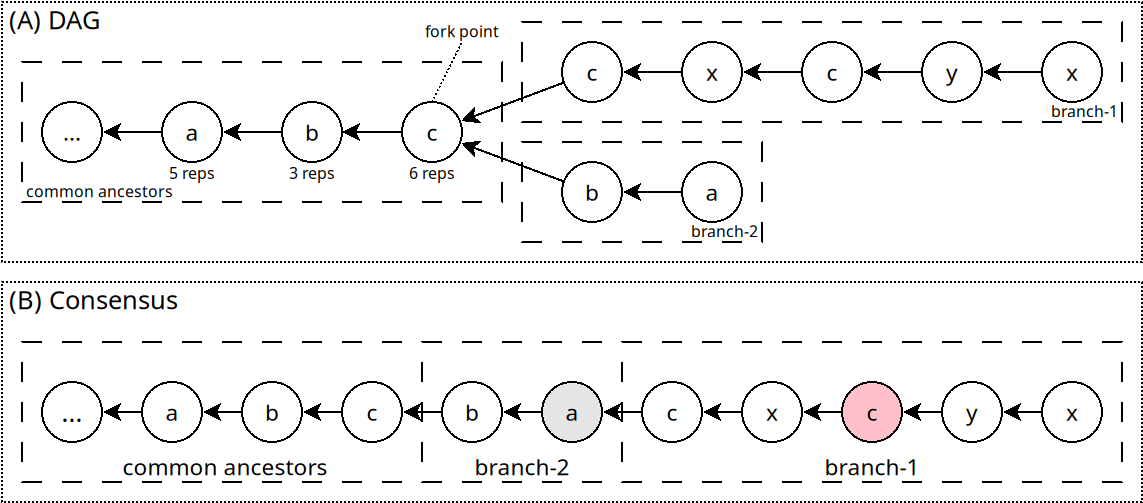
\includegraphics[width=0.85\textwidth]{dag.png}
\caption{
    (A) Forum DAG with common ancestors and two branches.
    (B) Total order after consensus.
}
\label{fig.reps}
\end{figure*}

Figure~\ref{fig.reps}.A illustrates a forum DAG forked by a temporary network
partition.
The common ancestors have signed actions from members $a$, $b$, and $c$.
Up to the fork point, we assume that members $a$ and $b$ have more
contributions in the prefix (omitted as \code{...}) and therefore hold more
\reps combined than $c$ has alone ($5+3>6$).
%
Then, member $c$ disconnects and keeps posting with new members $x$ and $y$ in
\code{branch-1}.
Meanwhile, $a$ and $b$ also participate with new posts in \code{branch-2}.
%
When the network reconnects and the DAG finally merges, we need to replay the
actions to check for inconsistencies.
Based on the reputation of the disjoint members up to the fork point,
Figure~\ref{fig.reps}.B indicates the resulting consensus order:
    first the common ancestors,
    then all actions in \code{branch-2},
    then all actions in \code{branch-1}.

During replay in consensus order, if any action fails (e.g., a double-spend),
then all remaining actions in the losing branch are rejected and erased from
the DAG, as if they never existed.
%
As an example, in Figure~\ref{fig.reps}.B, suppose that the last action by $a$
in \code{branch-2} (in gray) is a dislike to member $c$ that affects its
capacity to act in the forum.
Then, it is possible that the last post by $c$ in \code{branch-1} (in red) is
rejected together with all actions in sequence (since they cannot persist in the
Merkle~DAG).

We now recap the consensus mechanism and how it applies to
Figure~\ref{fig.reps}:
%
\begin{itemize}
\item Split members into disjoint sets at the fork point:   \\
    $M_1=\{c,x,y\}$ and $M_2=\{a,b\}$
\item Sum the \reps of each set in the common history:      \\
    $R_1=6$ and $R_2=8$
\item Order branches by highest sum first:%
\footnote{
    We compare the action hashes after the fork point as the tie breaker.
}                                                           \\
    \code{common <- branch-2 <- branch-1}
\item Discard actions from the first failure on:            \\
    \code{c <- y <- x}
\end{itemize}

Forks and merges raise a few other considerations.
%
Peers that first receive the branch with more reputation just append the other
branch, with no reordering and no extra effort.
This behavior is expected to happen on most peers.
%
However, the other side needs to reorder all actions after the fork point,
which might involve erasing content from the end-user software.
This behavior is similar to Bitcoin's blockchain reorganization, when peers
detect a new longest chain.
%
Legitimate actions that are erased must be reposted by their authors.
Still, we expect legitimate members to gossip among themselves more often,
which makes this situation rare.
%
Note that, unlike Bitcoin, forks are not only permitted but encouraged due to
the local-first software principle~\cite{p2p.local}.
However, the longer a peer remains disconnected, the higher the chances of
conflicting actions.
%
In summary,
    (i) forks and merges may introduce conflicts;
    (ii) conflicts require a consensus order to replay actions;
    (iii) the order is based on the reputation in the common history; and
    (iv) replay leads to a global and deterministic state.

\subsection{Network Partitions}
\label{sec.design.partitions}

Peer-to-peer networks have no dedicated infrastructure to keep connections
stable, especially under a permissionless regime, so partitions are not
exceptional events, but the norm:
    peers join, leave, and reconnect at will.
%
Partitions are also \emph{unbounded} and possibly \emph{malicious}, since a
peer may stay offline for as long as it wants, and no one can distinguish
whether the causes are deliberate or accidental.
%
Note that our local-first approach contrasts with standard blockchains, which
consider partitions as faults, and assume an online majority that discards
minority branches.

The protocol, therefore, cannot treat partitions as attacks, but can only
react to the damage they may cause.
Next, we discuss the threats and countermeasures under unbounded partitions:
%
\begin{description}
\item [\S\ref{sec.design.partitions.farming}]
    Reputation Farming:
    how an isolated branch mints \reps unchecked.
\item [\S\ref{sec.design.partitions.hardforks}]
    Hard Forks:
    how a settling window bounds the damage.
\end{description}

\subsubsection{Reputation Farming}
\label{sec.design.partitions.farming}

Consider a malicious scenario in which member $c$ in Figure~\ref{fig.reps}.A
intentionally disconnects from the network for weeks to cultivate fake
identities $x$ and $y$ that accumulate \reps from junk posts (\R{1.b}).
%
When merging, these fake members would become legitimate and take over the
majority of \reps in the forum.

\begin{lstlisting}[
    float=tbp,
    label={lst.discard},
    caption={Refuting a minority farming attack.}
]
# PEER A
$ fc /chat sync C                # receives branch-1
$ fc /chat discard 7c1e2a9       # drops branch-1
$ fc /chat dislike 5000 member c # tip of branch-2
$ fc /chat sync C                # merges again
$ fc /chat list order
...                              # branch-2
...                              # branch-1 missing
\end{lstlisting}

However, this attack is refutable: since the common history is the basis of
consensus, members in the branch with more reputation can still react, even
\emph{a posteriori}.
%
For instance, members $a$ and $b$ can pretend that they did not yet see
\code{branch-1} and post extra dislikes to member $c$ from \code{branch-2} so
that a further merge invalidates all actions from \code{branch-1}, as if they
never existed.
%
Listing~\ref{lst.discard} uses the \code{discard} command to drop the offending
\code{branch-1} locally before casting the dislike that bans $c$, so that the
next merge rejects \code{branch-1} for good.
%
Note that, as peers synchronize, all honest peers converge to the same state,
i.e., a single refutation propagates to the rest of the network.

Therefore, a minority attack that farms new \reps is refutable, since its
power is bounded by the \reps in the common history, but it requires the
intervention of at least one honest member.

\subsubsection{Hard Forks}
\label{sec.design.partitions.hardforks}

Considering that forging long branches from ancient fork points is
undetectable, reputation alone becomes a fragile criterion for consensus.
For instance, past members holding the majority of \reps at any point in time
could still override the present, which corresponds to the \emph{long-range
attack} in proof-of-stake~\cite{pos.weak}.

In Figure~\ref{fig.reps}.A, as a counterpoint to member $c$ farming \reps,
suppose members $a$ and $b$ are the ones who have abandoned the forum for
months, and thus \code{branch-1} is actually legitimate.
In this case, members $a$ and $b$ would succeed in taking over the forum,
since they control the majority of \reps in the common history.
%
Yet another possibility is that both branches are legitimate but were
genuinely disconnected for a long period.
In any case, it is unacceptable that an old remote branch affects an active
local forum.

\begin{figure}
\centering
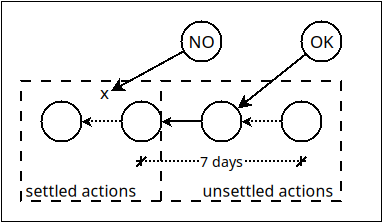
\includegraphics[width=0.3\textwidth]{hard.png}
\caption{
    Settled local branch with frozen actions.
}
\label{fig.hard}
\end{figure}

Therefore, as a measure against malicious members with strong past reputation,
\FC protects settled local branches from unexpected consensus reorderings,
which corresponds to checkpoints in proof-of-stake~\cite{pos.weak}.
%
As Figure~\ref{fig.hard} illustrates, actions older than the most recent 100
actions or 7 days are frozen and cannot be reordered.
If consensus would reorder them, the merge is refused and the two peers become
incompatible, which is analogous to a hard fork in Bitcoin.
In contrast, peers that remain active and synchronize over time evolve together
with a stable order.

In summary, the consensus rules to merge a local branch \code{i} with a remote
branch \code{j} are as follows:
\begin{itemize}
    \item \code{i} wins:
        \code{i} is first, \code{j} is second
        (same as \S\ref{sec.design.consensus}).
    \item \code{j} wins and \code{i} is unstable:
        \code{j} is first, \code{i} is second
        (same as \S\ref{sec.design.consensus}).
    \item \code{j} wins and \code{i} is stable:
        \code{i} is first, \code{j} is rejected
        (new hard fork rule).
\end{itemize}

To conclude, since consensus rests on subjective ratings, forks are legitimate
outcomes rather than failures.
Unlike Bitcoin, forums may split and diverge freely, and members may even fork
deliberately to ``reboot'' a community from a previous state.
%
The consensus algorithm does not prevent such splits, but makes them
transparent and deterministic, so that members understand the evolution of a
forum and act accordingly.
Ultimately, a hard fork is a social conflict, not a numeric dispute.

%%%%%%%%%%%%%%%%%%%%%%%%%%%%%%%%%%%%%%%%%%%%%%%%%%%%%%%%%%%%%%%%%%%%%%%%%%%%%%%

\iffalse

\item [\S\ref{sec.design.overall}]
    describes the overall reputation and consensus mechanism.
\item [\S\ref{sec.design.forks}]
    discusses malicious behaviors and hard forks.
\item [\S\ref{sec.design.time}]
    discusses timestamp convergence, regardless of local temporary time-based
    decisions.
\item [\S\ref{sec.design.revoke}]
    describes how members revoke abusive content.
\item [\S\ref{sec.design.algo}]
    details the consensus algorithm that orders actions.
\item [\S\ref{sec.design.byz}]
    discusses peer synchronization under Byzantine faults.
\fi

\iffalse
For instance, federated protocols explicitly leave SPAM filtering to the server
side~\cite{pubsub.activitypub}, while CRDT-based
systems~\cite{p2p.merkle-crdts,p2p.byz} assume honest replicas or only address
integrity, not volume or content quality.

Admitted posts reward authors with tokens they spend to rate other posts, a
\textbf{proof-of-authoring} in which generation is expensive and assessment
is cheap (akin to Bitcoin's mining).
Members rate and revoke posts as, which
preserves the Merkle DAG since payloads are referenced by hash.
A \textbf{permissionless Wiki} shows how consensus empowers mostly
conflict-free replicated data types (\emph{quasi-CRDTs}) by automating
merges of user-assessed edits.

We assume \emph{Carol} is honest and online...
Also, local time

In \FC, members may stay offline indefinitely without losing \reps, and both
sides of a partition remain legitimate forums while they last.
This is a deliberate choice of availability over consistency~\cite{cap}, at
the cost of a single global history: a long partition may end as a hard fork
rather than as a reorganization (\S\ref{sec.design.partitions.hardforks}).

Note that a dislike shrinks the forum economy, since it removes \reps from
both origin and target.
Hence, dislikes are meant to combat abuse, not to suppress divergence of
opinion.
Note also that rule~\code{4.b} limits members to at most \nreps{30}, which
provides incentives to spend likes and thus decentralize the network, while
rule~\code{4.c} limits the size of actions to at most \emph{128KB} to prevent
DDoS attacks using gigantic blocked actions.

Finally, the actual contents of a post may be revoked if it has at least 3
dislikes, and more dislikes than likes (rule~\code{3}).
However, considering that \reps are scarce, dislikes are encouraged to combat
abusive behavior, but not to eliminate divergences of opinion.

In summary, the reputation system makes \FC
**(a)** Sybil-resistant: write operations require and spend `reps`; and
**(b)** permissionless: any insider can transfer `reps` to welcome any outsider.

In this sense, having one or hundreds of machines in the network does not
affect the capacity to write into the forums.
We consider Sybils as groups of throw-away identities and machines with no
previous reputation in the forums.
In our analogy with Bitcoin, Sybil attacks would require to add human resources,
instead of CPU power.

), since it is the maximum information that all branches

According to \R{2}, only one of them should be accepted by the network.
However, without consensus, it is not possible to globally determine which one
to accept, since each peer would supposedly accept the first message it receives.
On the one hand, in order to validate operations consistently, we need the same
message ordering across all peers in the network.
On the other hand, due to network partitions, we can only represent public
forums as DAGs (directed acyclic graphs) with causal relationships between
messages, which provides at most partial order.

Going back to the malicious member example, the simultaneous messages would
appear as forks in the forum DAG.
Only the message in the fork with more combined work would be accepted, while
all other Sybil messages would be rejected.

Note that even non-malicious partitions may experience conflicts when
merging.
For instance, dislike operations in one branch to past actions in the common
prefix could possibly block actions from members in the other branch.
%, depending on how the actions are ordered.
Therefore, we need to order branches with a global consensus, such that we can
validate operations consistently across the network.
%
Note also that, to reach consensus, we should preferably rely on the maximum
information that all branches agree on, which is exactly the actions in the
common prefix.

\subsection{Public Forum Chains}
\label{sec.design.chains}

The most basic concern in forums is to resist Sybils abusing the
chains.
Fully peer-to-peer systems cannot rely on logins or {\footnotesize CAPTCHAs}
due to the lack of a central authority.
Viable alternatives include (i) building social trust graphs, in which members
already in the community vouch for new members, or (ii) imposing explicit costs
for new posts, such as proof of work.
%
We propose a mix between social trust graphs and explicit costs for new posts.
%
Rule~\code{4.a} requires that members have at least \nreps{500} to post,
effectively blocking Sybil actions.
To vouch for new members, rule~\code{3.a} allows an existing member to like a
newbie's post to unblock it, but at the cost of \nreps{500}.
This cost prevents malicious members to unblock new members indiscriminately,
which would be a breach for Sybils.
For the same reason, rule~\code{2} imposes a temporary cost of \nreps{500} for
each new post.
%
Note that the pioneers rule~\code{1.a} solves the chicken-and-egg problem
imposed by rule~\code{4.a}: if new members start with no \reps, but require
\reps to operate, it is necessary that some members have initial \reps to boot
the chains.

New posts penalize members with \nreps{-1} during at most 12 hours
(rule~\code{2}), which depends on the activity succeeding (and including) the
new post.
The more activity from reputed members, the less time the discount persists.
In the example, since the post is from the pioneer controlling all \reps in the
chain, the penalty falls immediately and she remains with \nreps{30}.
This mechanism limits the excess of posts in chains dynamically.
For instance, in slow technical mailing lists, it is more expensive to post
messages in sequence.
However, in chats with a lot of active members, the penalty can decrease to zero
quickly.

\subsection{Content Revocation}
\label{sec.design.revoke}

\begin{figure}
\centering
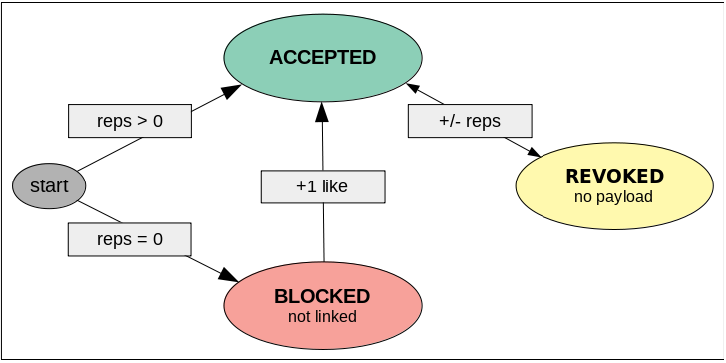
\includegraphics[width=0.49\textwidth]{state-revoked.png}
\caption{
    State machine of actions:
    \code{BLOCKED} actions are not linked in the DAG.
    \code{ACCEPTED} actions are linked and retransmitted.
    The payload of \code{REVOKED} actions are not retransmitted.
}
\label{fig.state}
\end{figure}

Finally, we consider that revoking posts is fundamental in the context of
social content publishing, and thus, an important contribution of this work.

An action has three possible states: \code{BLOCKED}, \code{ACCEPTED}, or
\code{REVOKED}.
Figure~\ref{fig.state} specifies the transitions between states.
%
If the member has reputation, a new action is immediately \code{ACCEPTED} in
the forum.
%
Otherwise, it is \code{BLOCKED} and requires a like from another member.

Blocked actions are not considered part of the forum DAG in the sense that new
actions do not link back to it.
In addition, peers are not required to hold blocked actions nor retransmit them
to other peers.
However, if blocked actions are not disseminated, new members will never have
the chance to be welcomed with a like.
Therefore, a reasonable policy is to hold blocked actions in a temporary bag
and retransmit them for some visibility.

Once accepted, the action becomes part of the forum and can never be removed
again, since Merkle~DAGs are immutable by design.
%Note that blocked actions that become accepted are always succeeded by a
%\emph{like} (Figure~\ref{fig.forum}).
%
However, if the number of dislikes exceeds an arbitrary threshold (e.g., more
dislikes than likes), the action becomes \code{REVOKED} and its payload is not
retransmitted to other peers.
Note that an action hash does not depend on its associated payload, but only on
the payload hash.
Hence, it is safe to remove the payload as long as one can prove its revoked
state.
Later, if the action receives new likes, it means that the payload is still
known somewhere and peers can request it when synchronizing again, since the
action becomes \code{ACCEPTED} again.

In summary, the operations and constraints in Table~\ref{tab.rules} together
with the consensus rules of Figures~\ref{fig.reps}~and~\ref{fig.hard} empower
\FC with permissionless public forums.

\subsection{The Consensus and Synchronization Algorithm}
\label{sec.design.algo}

In order to validate publications consistently across the network, the
consensus algorithm needs to execute at the core of the protocol, and at the
time peers synchronize their chain DAGs.
From the perspective of a peer on the receiving side, the overview of the
consensus and synchronization algorithm is as follows:
\begin{enumerate}
\item \textbf{Consensus:}
    Calculate the consensus order of actions considering the local DAG.
\item \textbf{Synchronization:}
    Receive the next missing action respecting topological order.
\item \textbf{Verification:}
    Verify that the action is valid and add it to the local DAG.
\item \textbf{Repeat:}
    Restart from step (a) until no actions are missing.
\end{enumerate}

Step (a) is discussed and motivated in extent in the previous sections.
The actual algorithm is detailed further and adapts topological sorting to
favor branches with more reputation.

Step (b) is very similar to a recent work on \emph{Byzantine Causal
Broadcast}~\cite{p2p.dag.sync}, which also synchronizes DAGs representing
causal messages:
% in the presence of malicious nodes:
    (i)   starting from the heads of the DAGs;
    (ii)  traverse each head backwards until a common action is found;
    (iii) now traverse forward all missing actions, respecting topological
          order;
    (iv)  each action represents an iteration of Step (b).
What distinguishes our algorithm is that \code{BLOCKED} actions are not
synchronized, which mitigates denial of service attacks with very long
malicious branches.
We also limit the number of iterations on Step (b.ii) to ensure that the
algorithm terminates.
If necessary, a remote peer that is disconnected for too long can try older
heads to adapt to this constraint.

Step (c) verifies if the next missing action found in Step (b) can be added to
the local DAG considering the consensus order found in Step (a).
It verifies the following properties:
    (i)   Merkle DAG structure is consistent (e.g., action hash and back
          pointers);
    (ii)  Back pointers are not in \emph{BLOCKED} state;
    (iii) Member signing the action has enough reputation.
In case of success, the action is added to the DAG and the next iteration of
the consensus algorithm already considers it.
Otherwise, the action is marked as \emph{BLOCKED}, and the remaining branch is
ignored in Step (b.iii).

The topological sorting for the Consensus Step (a) is an adaptation of Kahn's
algorithm~\cite{kahn}:
%
\begin{enumerate}
\item The set $S$ of all actions in the DAG with no incoming edges starts with
      the chain genesis.
\item Removes from $S$ the action $B$ in the branch with more reputation
      (Figure~\ref{fig.reps}) and adds it to the end of the consensus list $L$.
      (This is the only step that differs from Kahn's algorithm, which would
      take any action from $S$.)
\item Adds to $S$ all actions directly in front of $B$, excluding those
      reachable from any node still in $S$.
\item When $S$ is empty, the list $L$ holds the consensus order.
\end{enumerate}
%
Step (b) requires to find the maximum value in set $S$ according to the
reputation criteria.
The comparison function needs to find the non-common members in the suffix of
the two branches in order to compare the sum of their reputations.
%
For this reason, the algorithm also needs to track negative, neutral, and
positive actions according to Table~\ref{tab.rules}.
%
We take advantage of the hard fork rule that freezes the consensus list $L$
when crossing the activity threshold (stable consensus in Figure~\ref{fig.hard}).
We use it as a checkpoint to cache the reputations, which limits the input size
to a short fixed size that does not depend on arbitrary chain sizes.

Currently, we hold the DAG structure directly in the file system with no
database support.
Each chain uses a separate directory, and each action uses two separate files:
a \emph{JSON} for the metadata and a payload exactly as posted.
We save the cache and current consensus order in an index file.
We build the DAG by traversing the chain directory.

\subsection{Peer Synchronization and Byzantine Faults}
\label{sec.design.byz}

Similarly to Bitcoin, the underlying network protocol replicates on each peer
the full state of the Merkle~DAG representing the causal relationships between
actions.
When peers synchronize, they mutually exchange missing branches such that they
reach the same DAG structure~\cite{p2p.byz}.
As they synchronize, each peer runs the consensus algorithm locally and
verifies if all received actions are consistent.

Because the protocol relies on tamper-proof DAGs, and because each peer self
verifies the actions as they synchronize, the protocol becomes tolerant to
Byzantine faults~\cite{lamport.byz}.
%
Note that no information coming from any peer is trusted a priori.
%
For instance, a malicious peer that tries to synchronize branches with erratic
data can be detected on the first inconsistent action.
This allows the correct peer to close the connection immediately and blacklist
the malicious peer from future connections.

Therefore, although Byzantine peers may still perform some sort of denial of
service attacks in the network, they cannot modify the DAG structure, nor
create arbitrary content, nor impede that two correct nodes synchronize
directly.

\section{Experiments with Forum Archives}
\label{sec.evaluation}

We performed experiments to evaluate the performance of \FC and its consensus
algorithm.
%
As detailed next, we measure the following evaluation parameters:
    (a) metadata overhead,
    (b) consensus runtime,
    (c) graph forks, and
    (d) blocked messages.
%
Our goal is to stress the consensus algorithm to show that permissionless
public forums are viable, regardless of the inherent slower performance in
comparison to permissioned protocols.

We simulate the behavior of two publicly available forums as if they were using
\FC:
%
    a chat channel from the Wikimedia Foundation%
\footnote{ Chat: \url{https://archive.org/download/WikimediaIrcLogs/} }, and
    the \emph{comp.compilers} newsgroup%
\footnote{ Newsgroup: \url{https://archive.org/download/usenet-comp} }.
%
Chats and newsgroups represent typical public forums with
    faster interactions with shorter payloads (chats), and
    slower interactions with larger payloads (newsgroups).
%
We only simulate the first \emph{10.000} messages of the forums, which
represent 3 months of activity in the chat and 9 years in the newsgroup.

TODO: fazer para periodo inteiro, explicar pack do git

The simulation spawns $N$ peers, each joining the same chain with the same
arguments.
For each message in the original forum, we
    (i)   set the timestamp of peers to match the original date,
    (ii)  create a pair of keys if the member is new,
    (iii) post the message from a random peer in $N$,
    (iv)  like the post if the member has no reputation, and
    (v)   synchronize the chain with $M$ random peers.
%
Since all messages are part of the original archive, we always perform step
(iv) to unblock messages from newbies, which we also use to measure the
evaluation parameter (d): it counts extra likes to unblock existing users,
which could signal excessive bookkeeping in the chain.
Step (v) will inevitably create forks in the chain for any \texttt{M<N}, which
we measure in evaluation parameter (c).

For the newsgroup, we use \texttt{N=15} and \texttt{M=5}, which represents a
larger number of peers with few interconnections to stress the local-first
nature of the protocol.
For the chat, we use \texttt{N=5} and \texttt{M=3}, which is a smaller number
of peers but with more interconnections.
%
We executed each simulation $4$ times in a desktop PC (\texttt{i7} CPU,
\texttt{8GB} RAM, \texttt{512GB} SSD).
Since the variations were negligible, we always discuss the median measures.

\begin{comment}
We assume chats are less distributed given their real-time requirements, i.e.,
users would connect to a few but more interconnected peers.
Note that \FC focus on the decentralization of memberity, which is not directly
related to network distribution, which may vary from applications.
\end{comment}

Evaluation item (a) measures the protocol overhead due to blockchain metadata,
which consists of a timestamp, member signature, and hashes (action id,
payload, backlinks, and likes).
%
The original chat archive is \texttt{800kB} in size, or \texttt{80B} for each
message, which includes a timestamp, a username, and the actual payload.
The simulated chat chain is \texttt{8MB} in size, which indicates a $10x$
overhead.
% (\code{20100825 [03:37:43]})
% (\code{hello everyone})
% (\code{<Ashlee>})
The original newsgroup is \texttt{30MB} in size, or \texttt{3kB} for each
message, which includes a timestamp, a sender, a subject, and the actual
payload (typically much longer).
The simulated newsgroup chain is \texttt{42MB} in size, which indicates a
$50\%$ overhead.
% (\code{29 Aug 88 23:36:58 GMT})
% (\code{mark@ramid.com})
% (\code{Error messages and Yacc})
%
It is clear that the metatada overhead is not negligible, specially for short
chat messages, but decreases as the payload increases.

Evaluation item (b) accounts the consensus algorithm applied locally.
We measured the time to sort actions in a local DAG both for the first time,
and incrementally from stable consensus caches.
%
For the chat chain, it takes \texttt{125s} and \texttt{50ms} for the initial
and incremental sorts, while for the newsgroup chain, it takes
\texttt{100s} and \texttt{70ms}.
%
%Currently, we synchronize the DAGs takes hours because we the synchronization time
%
The incremental sort is limited to 7 days or 100 actions by design
(\S\ref{sec.design.overall}), regardless of the size of the chain,
which conveniently settles an upper bound on the input size of the consensus
algorithm.
%
Given that we use plain JSON files in the file system, we consider an
incremental consensus under \texttt{100ms} to be a practical upper bound.

Evaluation item (c) counts the number of forks in chain DAGs, which indicates
the level of asynchrony between peers following the local-first principle.
We calculate the ratio of forks over the total number of messages, e.g., a DAG
with $100$ messages and $10$ forks has a ratio of $10\%$.
%Based on the choices for $M$ and $N$ for each forum, we expect the newsgroup to
%have a higher ratio, since peers synchronize less.
We found a ratio of $18\%$ for the chat and $14\%$ for the newsgroup, which
confirms that the simulation achieves a reasonable level of asynchrony.

Evaluation item (d) measures how much bookkeeping is required to sustain active
members in the forums.
Even though the newbie rule~\code{4.a} in Table~\ref{tab.rules} is key to
combat Sybils, ideally it should not recurrently deny access to active members
with low reputation.
%
The evaluation counts the number of blocked messages requiring extra likes
after the welcoming likes (which are disconsidered) and calculates the ratio
over the total number of messages in the chain.
%This situation occurs when an user with low reputation tries to post multiple
%messages in a row without the necessary interval imposed by rule~\code{2}.
As an example, if $10$ members posted $110$ messages requiring $20$ likes, we
discount the $10$ initial messages and welcoming likes (when the member first
appears), and find a ratio of $10\%$ (\code{(20-10)/(110-10)}).
%
For the chat with $80$ members, we found a ratio of $3.7\%$.
For the newsgroup with $5000$ members, we found a ratio of $3.5\%$.
%
Considering that members were not aware of the reputation rules, the low ratios
indicate that their "natural" posting behavior matches the constraints of the
rules.
%As expected, the newsgroup has a lower bookkeeping given the higher interval
%between messages.
%
We assume that members would use the revoke mechanism to combat abusive content,
having no further effects on our evaluation.
%We also do not evaluate the quality of posts and how they would affect the
%reputation of users.

\begin{comment}
CHAT
timestamp user message
 798857 bytes

> DELL+ /x/tmp/fc-chat-20220529
- 3.7
- 455793 7419368 7875161
- erro (consensus ate 93\_*)
- 10491 / 1794 = 17%

> DELL+ /x/tmp/fc-chat-20220530
- 3.7
- 455793 7433845 7889638
- erro (consensus ate 93\_*)
- 10510 / 1851 = 18%

> DELL- /x/tmp/fc-chat-20220529
- 3.7
- 455793 7434379 7890172
- 125s, 50ms
- 10511 / 1852 = 18%

> DELL- /x/tmp/fc-chat-20220530
- 3.7
- 455793 7433590 7889383
- 150s, 50ms
- 10510 / 1850 = 18%

> NOTE 20220530
- 5.1
 455811
7577544
- 100ms / 130ms
- 10693 / 1811 = 17%

> NOTE 20220531
- 3.7
 455793
7434804
- 100ms / 130ms
- 10511 / 1851 = 18%

> NOTE 20220601
- 3.5
 455793
7384694
- 249s / 100ms
- 10456 / 1837 = 18%

-------------------------------------------------------------------------------

USENET
code From: Subject: Date: BODY
29.863.335 bytes

> DELL+ /x/tmp/fc-usenet-20220531
- 8.9
42.262.616
- 73s / 66ms
- 15659 / 2395

> DELL+ /x/tmp/fc-usenet-20220601
- 8.9
42357914
- 75s / 70ms
- 15682 / 2195

> DELL+ /x/tmp/fc-usenet-20220602
- 8.9
- 69s / 66ms
- 15669 / 2286

> DELL+ /x/tmp/fc-usenet-20220603
- 3.5
- 64s / 64ms
- 15416 / 2327

> DELL+ /x/tmp/fc-usenet-20220604
- 3.4
- 64s / 66ms
- 15419 / 2329

> DELL+ /x/tmp/fc-usenet-20220605
- 3.3
- 65s / 64ms
- 15391 / 2324

> DELL- /x/tmp/fc-usenet-20220601
- 8.7
42160398
- 52s / 70ms
- 15665 / 2198 = 14%

> DELL- /x/tmp/fc-usenet-20220602
- 60s / 70ms
- 15678 / 2091 = 13%

- lockdown strategy ok?

Discussion:
- do not scale
    - restart
- cannot evaluate behavior
    - dislike is immediate
- users are not aware of the policies
    -
- no images, videos
    - 128k enough for memes?

- Two cases
    - chat:
        - 2010-08-25 2012-11-01
        - 166277 messages
        - 13726470 bytes w/  metadata (date/time/user+msg)
        - 8592725 bytes w/o metadata (only msg)
        - 82/50 bytes/message (w/-w/o metadata)
        - 651 users
        - 227 messages per day

    - forum:
        - 1987-08-17 2012-05-28
        - 35366 messages
        - 117458214 bytes w/ metadata (date/time/user/*/+msg)
        - 3321 bytes/message
        - 13000 users
        - 3.8 messages per day

- number of forks
    - chat 30s per peer
    - e-mail 1h per peer
- time of consensus
\end{comment}

\section{Correspondences with CRDTs}
\label{sec.crdts}

Conflict-free replicated data types (CRDTs)~\cite{p2p.crdts} serve as a robust
foundation to model concurrent updates in collaborative local-first
applications~\cite{p2p.local}.
However, CRDTs are not a panacea and often require human intervention to solve
specific conflicts (\emph{quasi-CRDTs}), such as manual merges in version
control systems (VCSs).
%
Our observation is that, since the proposed consensus algorithm already relies
on human interactions, we can use it to resolve conflicts automatically.

We propose a three-layered CRDT scheme to build decentralized collaborative
applications:
    state-based CRDTs at transport layer (CvRDTs),
    operation-based CRDTs at application layer (CmRDTs), and
    quasi-CRDTs with arbitrary operations after consensus is applied.

At the transport layer, Merkle~DAG chains are trivial CvRDTs because they
converge to the same state on synchronization~\cite{p2p.merkle-crdts}.
%
At the application layer, however, DAGs loose this property because branches
might be processed in different orders across peers, resulting in incompatible
states.
An interesting approach is to require posts to represent commutative
operations, thus resulting in CmRDTs~\cite{p2p.merkle-crdts}.
%
CmRDTs have the advantage to store only small updates that are sufficient to
reconstruct any version of the data.
%This contrasts with CvRDTs, which would require to store complete versions.
%
At the third layer, the consensus algorithm transforms a chain DAG into a
totally-ordered set, which supports quasi-CRDTs with non-commutative
operations.
Note that even full-CRDTs can benefit from consensus, since they often
encounter corner cases that require arbitrary choices (e.g., aggregating
updates or ressurecting data~\cite{p2p.automerge}).

Next, we illustrate this three-layered CRDT scheme through an example of a
simple permissionless decentralized VCS (dVCS) implemented on top of public
chains.

\subsection{A dVCS with Automatic Merges}

We built a simple dVCS with the functionalities (and associated \FC
operations) as follows:
%
\begin{itemize}
    \setlength{\itemindent}{-8pt}
    \item initialize a repository (\code{join})
    \item commit local changes to repository (\code{post})
    \item checkout repository changes to local (\code{consensus/get})
    \item synchronize with remote peer (\code{send/recv})
    \item rate and revoke commits (\code{like/dislike})
\end{itemize}
%
The system relies on public forum chains, which means that repositories are
permissionless and adhere to the proposed reputation and consensus mechanism.
The main innovations in this system are that
    (i)  users can rate commits to reject them, and
    (ii) checkout operations resolve conflicts automatically based on consensus
         order.

As a concrete example, we model a Wiki article as a chain behaving as a VCS
holding its full edition history.
To model a complete Wiki platform, we assume that an article could refer to
other articles using hyperlinks to other chains.

Most VCS operations, except \code{commit} and \code{checkout}, map directly to
single \FC commands.
For instance, to create a repository, we simply join a public chain with the
name of the file we want to track.
In the commands that follow, we create a repository with multiple pioneers, and
then edit and commit the file twice:

{\footnotesize
\begin{verbatim}
 > freechains '#p2p.md' join A2885F.. 2B9C32..
 2F11BF..
 > echo "P2p networking is..." > p2p.md
 > freechains-vcs '#p2p.md' commit --sign=69929..
 1_4F3EE1..
 > echo "The [USENET](#usenet.md), ..." >> p2p.md
 > freechains-vcs '#p2p.md' commit --sign=69929..
 2_B58D22..
\end{verbatim}
}

The \code{commit} operation expands as follows:

{\footnotesize
\begin{verbatim}
 > freechains-vcs '#p2p.md' checkout p2p.remote
 > diff p2p.remote p2p.md > p2p.patch
 > freechains '#p2p.md' post p2p.patch --sign=69929..
\end{verbatim}
}

A commit first makes a checkout from the repository into temporary file
\code{p2p.remote}.
Then, it compares this version against our local changes, saving the diffs
into file \code{p2p.patch}.
A patch contains the minimal set of changes to apply back into the repository,
and represents a CmRDT operation in our model.
Finally, the commit posts the patch file back into the chain.
Evidently, the chain name and signature (\code{\#p2p.md} and \code{--sign=...})
are parameters in the actual implementation of \code{commit}.
The checkout operation is expanded further.

Much time later, the other pioneer synchronizes with us, checks out the file,
and then edits and commits it back:

{\footnotesize
\begin{verbatim}
 > freechains '#p2p.md' recv '<our-ip>'
 2/2    <-- two commits above
 > freechains-vcs '#p2p.md' checkout p2p.md
 > echo "P2P does not scale!" >> p2p.md
 > freechains-vcs '#p2p.md' commit --sign=320B5..
 3_AE3A1B..
\end{verbatim}
}

A \code{checkout} recreates the latest version of the file in the repository by
applying all patches since the genesis post.
Recall that each patch represents a CmRDT operation to recreate the final state
of the data.
The \code{checkout} expands as follows:

{\footnotesize
\begin{verbatim}
 > rm p2p.md && touch p2p.md
 > for blk in `freechains '#p2p.md' consensus` do
    freechains '#p2p.md' get payload $blk > p2p.patch
    patch p2p.md p2p.patch
    if [ $? != 0 ]; then
     echo $blk  <-- hash of failing patch
     break      <-- ignore remaining patches
    fi
  done
\end{verbatim}
}

The \code{consensus} operation of \FC returns all hashes since
the genesis post, respecting the consensus order.
The loop reads each of the payloads representing the patches and apply them in
order to recreate the file.
If any of the patches fail, the command exhibits the hash of the offending
post and terminates.
We discuss this behavior further, when we illustrate commit conflicts.

Since the last commit above is clearly wrong (P2P networks do scale!), other
members in the network will dislike it until the post becomes
\code{REVOKED} in the chain: % (as described before in Figure~\ref{fig.state}):

{\footnotesize
\begin{verbatim}
 > freechains '#p2p.md' dislike 3_AE3A1B.. --sign=USR1
 > freechains '#p2p.md' dislike 3_AE3A1B.. --sign=USR2
 > freechains '#p2p.md' dislike 3_AE3A1B.. --sign=USR3
 > freechains-vcs '#p2p.md' checkout p2p.md
 > cat p2p.md
 P2p networking is...
 The [USENET](#usenet.md), ...  <-- no 3rd line
\end{verbatim}
}

This way, the checkout operation above will apply an empty patch associated
with the revoked post, effectively removing the wrong line from the file.
This mechanism illustrates how the reputation system enables collaborative
permissionless edition and curation.

Next, we create a conflicting situation in which two members edit and commit
the same line of the file concurrently:

{\footnotesize
\begin{verbatim}
 # PEER A (more reputation):
 > sed -i 's/P2p/P2P/g' p2p.md    <-- fix typo
 > freechains-vcs '#p2p.md' commit --sign=69929..
 4_A..

 # PEER B (less reputation):
 > sed -i 's/networking/computing/g' p2p.md
 > freechains-vcs '#p2p.md' commit --sign=320B5..
 4_B..

 # SYNCHRONIZE (exchange conflicting forks):
 > freechains '#p2p.md' recv '<our-ip>'
 1 / 1
 > freechains '#p2p.md' send '<our-ip>'
 1 / 1
 > freechains-vcs '#p2p.md' checkout p2p.md
 1 hunk FAILED -- saving rejects to file p2p.md.rej
 4_B..
 > cat p2p.md
 P2P networking is... <-- typo fixed (not computing)
 The [USENET](#usenet.md), ...
\end{verbatim}
}

After they commit the conflicting changes, the peers synchronize in both
directions and reach the state of Figure~\ref{fig.conflict}.
When we checkout the file, the patches are applied respecting the consensus
order.
As a result, we see that the first branch is applied, but not the second,
leaving the file in the longest possible consistent state.
%
This happens because of the \code{break} in the checkout operation:
once a conflict is found, no further patches apply in any of the remaining
branches.
%
We chose to adopt a \emph{first write wins} resolution to favor work in the
branches with more reputation.
Nevertheless, the failing patch branch is not totally ignored, since the
checkout saves the conflict file and indicates the post causing it.
%
We believe this optimistic choice that does not reject both patches is the most
advantageous, since it keeps the file in an usable state and warns about the
conflict to resolve.
For instance, the members can later decide to dislike one of the two commits to
revoke it and remove the warning.

\begin{figure}
\centering
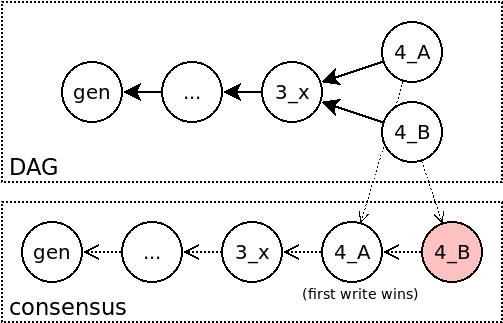
\includegraphics[width=0.35\textwidth]{conflict.png}
\caption{
    The branches in the DAG are ordered by reputation.
    Only the first patch is applied successfully (first write wins).
}
\label{fig.conflict}
\end{figure}

\subsection{Discussion}

In summary, the proposed reputation and consensus mechanism empowers a simple
dVCS with cooperative authoring and automatic conflict resolution.
It only requires the standard \emph{diff \& patch} tools and the basic API of
\FC.

We apply the proposed three-layered CRDT scheme as follows:
The first layer transports the whole commit history of small patches as a CvRDT
between peers, which eventually reach the same DAG state.
At this layer, the DAG is just raw data with no attached semantics.
%
In the second layer, peers need to interpret the DAG as a CmRDT of small
editions to recreate the file.
The \emph{patch} tool is mostly commutative, except when branches modify the
same lines.
%
Hence, in these situations, we resort to the third layer with the consensus
order, and apply the patches sequentially until a conflict occurs.
The final state of the file is guaranteed to be consistent, i.e., the result of
a sequence of correct patch applications.

\begin{comment}
Applications that rely only on commutative operations can traverse the DAG in
any causal order, possibly in parallel.
This is the case of most social apps with threaded conversations, in which
branches typically do not interfere with each other.
For instance, it is not problematic to rely on action timestamps to display
messages in chats, forums, and social media posts.
This is also the general case for notifications in these applications, such as
status updates and social engagements.
\end{comment}

Towards richer decentralized collaborative applications, we can employ CRDTs to
model data other than raw text.
As an example, \emph{Automerge}~\cite{p2p.automerge} manipulates JSON objects,
which supports non-trivial datasets with robust merging policies, but which
could still benefit from consensus to resolve corner cases.

\section{Related Work}
\label{sec.related}

% >>> TODO: moved from intro to related work
Permissionless consensus is notably challenging to the point that protocols
partially abdicate it along two axes.
%
On the one hand, \emph{multi-user/single-node consensus} supports a consistent
multi-user public forum, but restricted to a single trusted server ordering
messages (e.g., federated protocols~\cite{p2p.ecosystem}).
%
On the other hand, \emph{single-user/multi-node consensus} supports a
consistent feed across multiple machines, but restricted to a single author
ordering messages (e.g., Scuttlebutt~\cite{p2p.scuttlebutt}).
%
Our goal, therefore, is to support \emph{multi-user/multi-node consensus} in
the context of peer-to-peer public forums, i.e., a permissionless counterpart
of IRC/Discord or Usenet/Reddit.
% <<<

Many other systems have been proposed for decentralized content
sharing~\cite{p2p.survey,p2p.ecosystem}.
Here we consider the classes of publish-subscribe, federated, and peer-to-peer
protocols.

\subsection{Publish-Subscribe Protocols}

Decentralized topic-based publish-subscribe protocols, such as
    \emph{XMPP}~\cite{pubsub.xmpp},
    \emph{ActivityPub}~\cite{pubsub.activitypub}, and
    \emph{gossipsub}~\cite{pubsub.gossipsub},
decouples publishers from subscribers in the network.
%
A key limitation of \emph{pubsubs} is that the brokers that mediate
communication still have a special role in the network, such as authenticating
and validating actions.
%
Nevertheless, some pubsubs do not rely on server roles, and instead, use
peer-to-peer gossip dissemination~\cite{pubsub.tera,pubsub.rappel,pubsub.stan,pubsub.vitis,pubsub.gossipsub,pubsub.rappel}.
Most of these protocols focus on techniques to achieve scalability and
performance, such as throughput, load balancing, and real-time relaying.

However, these techniques alone are not sufficient to operate permissionless
networks with malicious Sybils~\cite{pubsub.gossipsub2}.
Being generic protocols, pubsubs are typically unaware of the applications
built on top of them.
%
In contrast, as stated in Section~\ref{sec.freechains}, the gossip layer of
\FC is conceptually at the application level and is integrated with the
semantics of chains, which already verifies actions at publishing time.
For instance, to flood the network with posts, malicious peers need to spend
reputation, which takes hours to recharge (rule~\code{2} in
Table~\ref{tab.rules}).
In addition, blocked actions (Figure~\ref{fig.state}) are not a concern either,
because they have limited reachability.
Another advantage of a tighter integration between the application and protocol
is that Merkle~DAGs simplify synchronization, provide persistence, and prevent
duplication of messages.
Full persistence resists long churn periods, and de-duplication tolerates
CmRDTs with operations that are not idempotent.

In summary, \FC and \emph{pubsub} middlewares operate at different network
layers, which suggests that \FC could benefit of the latter to manage the
interconnections between peers.

\subsection{Federated Protocols}
s
Federated protocols, such as e-mail, allow users from one domain to exchange
messages with users of other domains seamlessly.
\emph{Diaspora}, \emph{Matrix}, and \emph{Mastodon} are recent federations for
social media, chat, and microblogging~\cite{p2p.ecosystem}, respectively.

As a drawback, identities in federations are not portable across domains, which
may become a problem when servers shutdown or users become unsatisfied with the
service~\cite{fed.distributed}.
In any of these cases, users have to grab their content, move to another
server, and announce a new identity to followers.

Moderation is also a major concern in federations~\cite{p2p.ecosystem}.
As an example, messages crossing domain boundaries may be subject to different
policies that might affect delivery.
With no coordinated consensus, it is difficult to make pervasive public forums
practical.
%
For this reason, Matrix supports a permissioned moderation system%
\footnote{Matrix moderation: \url{https://matrix.org/docs/guides/moderation}},
but which applies only within clients, after the messages have already been
flooded in the network.

As a counterpoint, federated protocols seem to be more appropriate for
real-time applications such as large chats rooms.
The number of hops and header overhead can be much smaller in client-server
architectures compared to peer-to-peer systems, which typically include message
signing, hash linking, and extra verification rules (\S\ref{sec.evaluation}).

\subsection{Peer-to-Peer Protocols}

Bitcoin~\cite{p2p.bitcoin} is probably the most successful permissionless
network, but serves specifically for electronic cash.
IPFS~\cite{p2p.ipfs} and Dat~\cite{p2p.dat} are data-centric protocols for
hosting large files and applications, respectively.
Scuttlebutt~\cite{p2p.scuttlebutt} and Aether~\cite{p2p.ecosystem} are closer
to \FC goals and cover human communication.

Bitcoin adopts proof-of-work to achieve consensus, which does not solve the
centralization issue entirely, given the high costs of equipment and energy.
Proof-of-stake is a prominent alternative~\cite{p2p.proofs} that acknowledges
that centralization is inevitable, and thus uses a function of time and wealth
to elect peers to mint new blocks.
As an advantage, these proof mechanisms are generic and apply to multiple
domains, since they depend on extrinsic resources.
% (i.e., the richer gets richer)
In contrast, we chose an intrinsic resource, which is authored content in the
chains themselves.
We believe that human work grows more linearly with effort and is not directly
portable across chains with different topics.
These hypotheses support the intended decentralization of our system.
%
Another distinction is that generic public ledgers require permanent
connectivity to avoid forks, which opposes our local-first principle.
This is because a token transaction only has value as part of the longest
chain.
This is not the case for a local message exchange between friends, which has
value in itself.

IPFS~\cite{p2p.ipfs} is centered around immutable content-addressed data, while
Dat~\cite{p2p.dat} around mutable pubkey-addressed data.
IPFS is more suitable to share large and stable content such as movies and
archives, while Dat is more suitable for dynamic content such as web apps.
%
Both IPFS and Dat use DHTs as their underlying architectures, which are optimal
to serve large and popular content, but not for search and discovery.
In both cases, users need to know in advance what they want, such as the exact
link to a movie or a particular identity in the network.
%
On the one hand, DHTs are probably not the best architecture to model
decentralized human communication with continuous feed updates.
On the other hand, replicating large files across the network in Merkle~DAGs is
also impractical.
An alternative is to use DHT links in Merkle payloads to benefit from both
architectures.

Scuttlebutt~\cite{p2p.scuttlebutt} is designed around public identities that
follow each other to form a graph of connections.
This graph is replicated in the network topology as well as in data storage.
For instance, if identity $A$ follows identity $B$, it means that the computer
of $A$ connects to $B$'s in a few hops and also that it stores all of his posts
locally.
Note however that the basic unit of communication in Scuttlebutt is
unidirectional, with a public identity broadcasting a feed to its
followers (\Xon).
%
For open groups communication (\Xnn), Scuttlebutt uses the concept of channels,
which are in fact nothing more than hash tags (e.g. \emph{\#sports}).
Members can tag posts, which appear not only in their feeds but also in local
virtual feeds representing these channels.
However, users only see channel posts from members they already follow.
In practice, channels simply merge friends posts and filter them by tags.
In theory, to read all posts of a channel, a user would need to follow all
users in the network (which also implies storing their feeds).
A limitation of this model is that new users struggle to integrate in channel
communities because their posts have no visibility at all.
As a counterpoint, channels are safe places that do not suffer from abuse.

Aether~\cite{p2p.ecosystem} provides peer-to-peer public communities aligned
with \FC (\Xnn).
A fundamental difference is that Aether is designed for ephemeral, mutable
posts with no intention to enforce global consensus across peers.
Aether employs a very pragmatic approach to mitigate abuse in forums.
It uses established techniques, such as proof-of-work to combat SPAM, and an
innovative voting system to moderate forums, but which affects local instances
only.
In contrast, \FC relies on its permissionless reputation and consensus
mechanisms for moderation.

Regarding the structure of messages, append-only Merkle~DAGs have been proposed
as self-certified archives, and as CRDTs that provide strong eventual
consistency~\cite{fed.matrix,p2p.byz}.
However, when these DAGs are open to permissionless writes, they are subject to
abuse, which may degrade the content and performance of the network.
Another aspect is that a DAG itself has no attached semantics, which weakens
its consistency property at the application level, which may interpret the DAG
in conflicting orders.
The proposed consensus mechanism addresses permissionless writes and provides
a total order for applications (at the cost of rollbacks).

A similar dVCS have been recently proposed~\cite{p2p.dvcs}, with a DAG
representation and merging policies.
To resolve \emph{competition conflicts}, they propose to use an external
scoring function, such as users' reputations.
Our proposed consensus mechanism internalizes such reputation scoring function.
Integrated reputation also prevents SPAM and abusive behavior from byzantine
nodes, which could otherwise generate very large graphs that take forever to
synchronize (as discussed for Byzantine Causal Broadcast~\cite{p2p.dag.sync}).

Some works for P2P file sharing propose to account the reputation of peers to
form a web of trust based on their behavior
history~\cite{p2p.rep.wang,p2p.rep.eigentrust}.
However, there are three key aspects in terms of scope that distinguishes our
reputation system: its focus on the contents, its subjective nature, and its
dependency on consensus.
First, it is the actual contents that are stored and evaluated in the forums,
with the identities being a secondary attribute.
Second, content evaluation is subjective, as well as any decision to revoke
posts or to fork forums.
Third, at any given point in time, peers must agree on a common forum DAG
prefix with global and deterministic accuracy to act identically as a whole.
In this case, consensus is fundamental, since a subtle off-by-one discrepancy
in reputation creates an irreconcilable fork in the network.
Achieving consensus on a permissionless network is the key contribution of this
work.

\section{Conclusion}
\label{sec.conclusion}

In this paper, we propose a permissionless consensus and reputation mechanism
for social content sharing in peer-to-peer networks.
We enumerate four main contributions:
    (i)   human authored content as a scarce resource
          (\emph{proof-of-authoring});
    (ii)  diversified public forums, each as an independent blockchain with
          subjective moderation rules;
    (iii) abusive content removal preserving data integrity; and
    (iv)  three-layered CRDTs to build collaborative applications.

The key insight of the consensus mechanism is to use the human authoring
ability as a scarce resource to determine consensus.
This contrasts with extrinsic resources, such as CPU power, which are
dispendious and not evenly distributed among people.
%
Consensus is backed by a reputation system in which members can rate posts with
likes and dislikes, which transfer reputation between them.
The only way to forge reputation is by authoring new content under the
judgement of other members.
This way, reputation generation is expensive, while verification is cheap and
decentralized.

The reputation and consensus mechanism is integrated into \FC, a peer-to-peer
protocol, in which members can create public forums of interest and apply diverse
moderation policies.
In particular, members can revoke content considered abusive according to the
majority, not depending on centralized authorities.
%
We simulate the behavior of existing chat and newsgroup forums as if they were
using \FC to show the practicability of the protocol as a descentralized
alternative for public forums.

On top of the proposed three-layered CRDT architecture, we prototyped a
decentralized version control system that resolves commit conflicts
automatically:
    (i)   at the transport layer, the full commit history is held in a
          Merkle~DAG counting as a CvRDT;
    (ii)  at the application layer, the commit patches operate as (mostly)
          commutative CmRDT operations; and
    (iii) after consensus is applied, merge conflicts are resolved
          automatically.

Finally, we do not claim that the proposed reputation system enforces ``good''
human behavior in any way.
Instead, it provides a transparent and quantitative mechanism to help members
understand the evolution of forums and act accordingly.
Human creativity contrasts with plain economic resources (e.g.,
proof-of-work), which do not appraise social interactions and also tend
to concentrate power over the time.

\fi

\bibliographystyle{plain}
\bibliography{main}

\end{document}
